\section{Analysis}
\FloatBarrier % Now figures cannot float above section title

\subsection*{a}
Using the data in Table 2, the force vs deformation plot can be derived as \autoref{f3}. Also, from the lecture in week 7, we can learn that the total bending moment diagram is as follows


\begin{figure}[htbp]
    \centering
    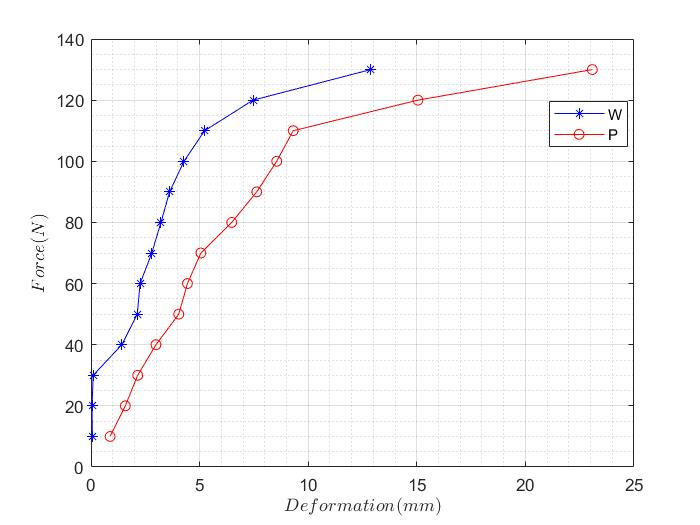
\includegraphics[width=9cm]{./fig/17.jpg}
    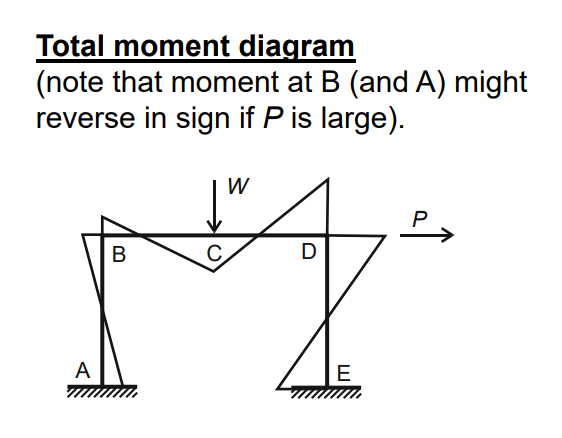
\includegraphics[width=7cm]{./fig/16.png}
    \caption{Force vs deformation and total moment diagram}
    \label{f3}
\end{figure}


The chart illustrates the relationship between the strength and deformation of steel, which can be discussed in two different situation.

$\bullet$ W<120N,P<110N: Elastic deformation: The relationship between the elastic deformation variable and the external force is linear.

$\bullet$ W$\geq$120N,P$\geq$110N: Plastic deformation: The relationship between force and deformation is nonlinear, i.e., the strain shows a rapid increase with the increase of stress.

From the total moment diagram (\autoref{f3}), it can be seen that the bending moment at point D is the largest, and this point will be the first point in the experiment to achieve plastic deformation.

In \autoref{f2}, The P-W graph is piecewise and if the combination of the P and W exceeds the closed figure on the left, The collapse will happen. In this case$(y=x)$, the collapse load for the frame was $W=148.63N,P=148.63N$.





